\iffalse
For AD progression prediction using longitudinal phenotypic markers, the input imaging features are a set of matrices X = {X1, X2, . . . , XT } ∈ Rd×n×T corresponding to the measurements at T consecutive time points, where Xt is the phenotypic measurements for a certain type of imaging markers, such as voxel-based morphometry (VBM) markers (see details in Section 3) used in this study, at time t (1 ≤ t ≤ T ).
\fi

\section{The Dataset and Problem Formalization}
\subsection{Datasets}
We obtained the data used in this experiment from the ADNI database~\cite{risacher2010longitudinal}. We downloaded 1.5 T MRI scans, single nucleotide polymorphisms (SNPs), and demographic information (age and gender) of 821 ADNI-1 participants. For the SNPs data, the quality control steps discussed in~\cite{shen2010whole} were followed, and 1223 SNPs for each participant are extracted. We performed voxel-based morphometry (VBM) and FreeSurfer (FS) on the MRI data following~\cite{risacher2010longitudinal} and extracted mean modulated gray matter measures for 90 target regions of interest. We also downloaded the longitudinal scores of the participants in five independent cognitive assessments including Alzheimer’s Disease Assessment Scale (ADAS), Mini-Mental State Examination (MMSE), Fluency test (FLU), Rey’s Auditory Verbal Learning Test (RAVLT) and Trail making test (TRAILS). 
% We also downloaded the longitudinal scores of the participants in five independent cognitive assessments including Alzheimer’s Disease Assessment Scale (ADAS)~\cite{rosen1984new}, Mini-Mental State Examination (MMSE)~\cite{tombaugh1992mini}, Fluency test (FLU)~\cite{ruff1987ruff}, Rey’s Auditory Verbal Learning Test (RAVLT)~\cite{moradi2017rey} and Trail making test (TRAILS)~\cite{reitan1958validity}. 
% Details about these cognitive assessments are available in the ADNI procedure manuals\footnote{http://adni.loni.usc.edu/wp-content/uploads/2010/09/ADNI\_GeneralProceduresManual.pdf}. 
In this analysis, the time points for both imaging records and cognitive assessments include baseline (BL), month 6 (M6), month 12 (M12), month 18 (M18), and month 24 (M24). We use the diagnosis at month 36 (M36) in Alzheimer's disease (AD), mild cognitive impairment (MCI), and healthy control(HC) as predictive target in our studies. The participants with no missing SNPs, demographic information, and AD diagnosis at M36 were included, providing a set of 379 subjects (104 AD, 115 MCI, 160 HC). The studied cohort includes 231 male and 148 female participants, and the average age is 75.35.
% Why multi class?

In the following pages, we denote a vector as a bold lower case letter, and a matrix as a bold upper case letter. For the arbitrary matrix $\mathbf{X}$, $[\mathbf{X}]^r$, $[\mathbf{X}]_c$, $[\mathbf{X}]^r_c$ denotes the $r$-th row, $c$-th column, an element of $r$-th row and $c$-th column respectively. We use $i$ and $j$ to index the participant and record respectively. We describe the records of the $i$-th participant as $\mathcal{X}_i = \{\mathbf{x}_i^b, \mathbf{x}_i^s, \mathbf{X}_i, \mathbf{M}_i, \mathbf{t}_i\}$. $\mathbf{x}_i^b \in \Re^{D_b}$ is a vector of basic demographic information (age and gender, $D_b = 2$), $\mathbf{x}_i^s \in \Re^{D_s}$ is a vector of SNPs ($D_s = 1223$), and $\mathbf{X}_i = [\mathbf{x}_i^1; \mathbf{x}_i^2; \cdots; \mathbf{x}_i^{n_i}] \in \Re^{n_i \times D_l}$ are the longitudinal records collected across the $n_i$ time points. $\mathbf{M}_i = [\mathbf{m}_i^1; \mathbf{m}_i^2; \cdots; \mathbf{m}_i^{n_i}] \in \{1, 0\}^{n_i \times D_l}$ are the binary masks of longitudinal records $\mathbf{X}_i$, where 1 and 0 indicates the observed and unobserved entry. Each longitudinal record at the $j$-th time point $\mathbf{x}_i^j$ ($1 \leq j \leq n_i$) is the concatenation of multi-modal neuroimagings and cognitive assessments, such that $\mathbf{x}_i^j = $ $[\mathbf{x}_{i,VBM}^j$, $\mathbf{x}_{i,FS}^j,$ $\mathbf{x}_{i,ADAS}^j,$ $\mathbf{x}_{i,MMSE}^j,$ $\mathbf{x}_{i,FLU}^j,$ $\mathbf{x}_{i,RAVLT}^j,$ $\mathbf{x}_{i,TRAILS}^j] \in \Re^{D_l}$, and the missing records are filled with the constant $-1$. $\mathbf{t}_i = [t_i^1; t_i^2; \cdots; t_i^{n_i}] \in \Re^{n_i}$ are the time stamps of $n_i$ records. The target label $\mathbf{y}_i \in \Re^{D_y}$ of the $i$-th participant is given for training if that participant is in training set, such that $i \in \Omega_{train}$. 
% The target label is one-hot encoded, such that $[1, 0, 0]$, $[0, 1, 0]$, and $[0, 0, 1]$ represent AD, MCI, and HC respectively. 
The input and output of the proposed model is described in Fig.~\ref{fig: final-inputs}.
\begin{figure}
    \centering
    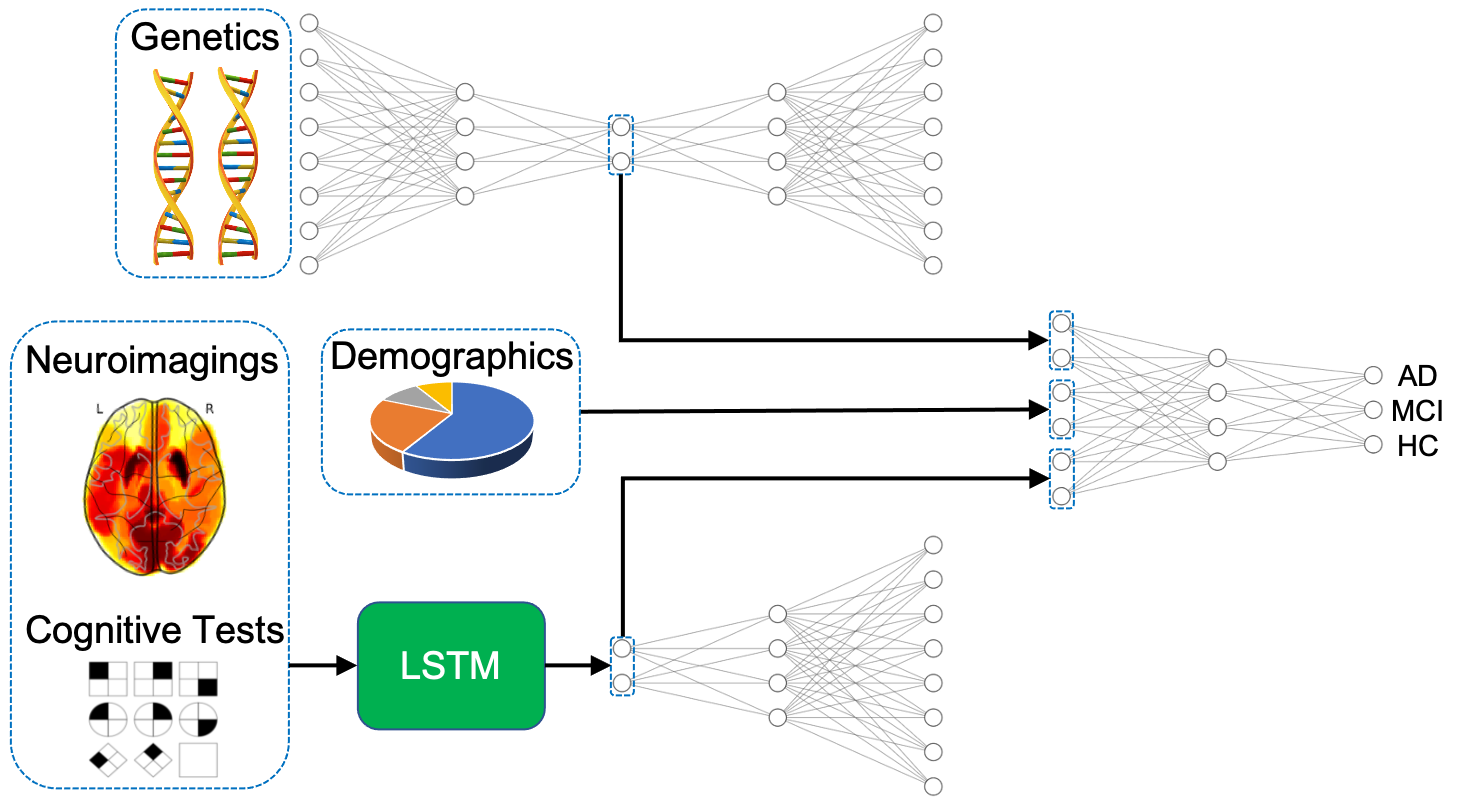
\includegraphics[width=0.95\textwidth]{images/final-inputs.png}
    \caption{Armed with the enriched representations of dynamic and static data, we can fully utilize the information in the dataset. 
    % The demographic information is provided without enrichment, as it's dimensionality is relatively small.
    } \label{fig: final-inputs}
\end{figure}

\subsection{Enrichment and Objective Formulation}
\subsubsection{Static Data Enrichment}
We leverage the autoencoder~\cite{kramer1991nonlinear} to learn the enriched representation of genotypic biomarkers. The autoencoder consists of two deep neural networks: an encoder $\phi_{SNP}: \Re^{D_s} \mapsto \Re^{d_s}$ that encodes a vector of SNPs into the enriched representation such that $\phi_{SNP}(\mathbf{x}_i^s;\ \theta^s_{E}) = \mathbf{z}_i^s$, and an decoder $\psi_{SNP}: \Re^{d_s} \mapsto \Re^{D_s}$ that decodes the enriched representation into the reconstructed vector of SNPs such that $\psi_{SNP}(\mathbf{z}_i^s;\ \theta^s_{D}) = \tilde{\mathbf{x}}_i^s$. $\theta_{E}^s$ and $\theta_{D}^s$ is the set of trainable weights matrices and bias vectors for the encoder and decoder respectively. 
% The deep neural network is defined as the $K$ consecutive fully connected layers where the output of the $k$-th layer is:
% \begin{equation}
%     \mathbf{h}_k = \sigma(\mathbf{h}_{k-1}\mathbf{W}_k + \mathbf{b}_k),
% \end{equation}
% where $\sigma$ is an activation function.
% The input $\mathbf{h}_0$ of the network is then forwarded to the last layer $\mathbf{h}_K = \tilde{\mathbf{x}}_i^s$, which is the output of the network. 
The encoded representation $\mathbf{z}_i^s$ preserves as much information as possible while removing the redundant noises in SNPs $\mathbf{x}_i^s$ by updating $\theta_{E}^s$ or $\theta_{D}^s$ to minimize the following reconstruction loss:
\begin{equation}
    \mathcal{L}_{static}(\mathbf{x}_i^s, \tilde{\mathbf{x}}_i^s;\ \theta_{E}^s, \theta_{D}^s) = \left\|\mathbf{x}_i^s - \tilde{\mathbf{x}}_i^s\right\|_F^2,
\end{equation}
where squared Frobenious norm $\| \cdot \|_F^2$ is summation of all the entries squared.

% then combining it with age and cognitive measures.
% Our models summarizes the dynamic and static data into a fixed-length vectorial representation.
% We use Long Short Term Memory (LSTM) architecture to learn the fixed-length vectorial abstract representation summarizing the incomplete time series with varying length and uneven time intervals.
% [In this section, we describe the semi-supervised AutoEncoder (AE) structure to learn a fixed-length vectorial representation for each patient's longitudinal records with varying length. The proposed AE is a composite model of three components. The encoder $\phi_E$ learns an abstract enriched representation of the input time series data. The decoder $\phi_D$ learns the reconstruction system to estimate the original data from the enriched representation. The predictor $\phi_P$ learns the prediction system to estimate the target labels from the enriched representation.].

\subsubsection{Dynamic Data Enrichment}
LSTM encoder $\phi_{dynamic}: \Re^{n_i \times (2 D_l + 1)} \mapsto \Re^{d_l}$ summarizes the longitudinal records $\mathbf{X}_i$ in the fixed-length vector $\mathbf{z}_i^l$. The time stamp of each record is crucial in learning the temporal relation (e.g. temporal locality) between records, and the pattern of missing entries may help the encoder to interpret the input. Thus we provide the concatenation of longitudinal records, masks, and time stamps, $[\mathbf{X}_i, \mathbf{M}_i, \mathbf{t}_i] = [\hat{\mathbf{x}}_i^1; \hat{\mathbf{x}}_i^2; \cdots; \hat{\mathbf{x}}_i^{n_i}] = \hat{\mathbf{X}}_i \in \Re^{n_i \times (2 D_l + 1)}$, as an input of the LSTM encoder such that $\phi_{dynamic}(\mathbf{X}_i, \mathbf{M}_i, \mathbf{t}_i;\ \theta_{E}^l) = \mathbf{z}_i^l$. 

The concatenated longitudinal record at the $j$-th time step $\hat{\mathbf{x}}_i^j$ ($1 \leq j \leq n_i$) is processed by the following LSTM architecture~\cite{yu2019review}:
\begin{equation}
    \mathbf{k}^j_i = \sigma(\hat{\mathbf{x}}^j_i \mathbf{W}_{xk} + \mathbf{h}_i^{j-1} \mathbf{W}_{hk} + \mathbf{c}_i^{j-1} \mathbf{W}_{ck} + \mathbf{b}_k),
\end{equation}
\begin{equation}
    \mathbf{f}^j_i = \sigma(\hat{\mathbf{x}}^j_i \mathbf{W}_{xf} + \mathbf{h}^{j-1}_i \mathbf{W}_{hf} + \mathbf{c}^{j-1}_i \mathbf{W}_{cf} + \mathbf{b}_f),
\end{equation}
\begin{equation}
    \mathbf{c}^j_i = \mathbf{f}^j_i \odot \mathbf{c}^{j-1}_i + \mathbf{k}^j_i \odot \operatorname{tanh}(\hat{\mathbf{x}}_i^j \mathbf{W}_{xc} + \mathbf{h}^{j - 1}_i \mathbf{W}_{hc} + \mathbf{b}_c),
\end{equation}
\begin{equation}
    \mathbf{o}^j_i = \sigma(\hat{\mathbf{x}}_i^j \mathbf{W}_{xo} + \mathbf{h}^{j-1}_i \mathbf{W}_{ho} + \mathbf{c}^j_i \mathbf{W}_{co} + \mathbf{b}_o),
\end{equation}
\begin{equation}
    \mathbf{h}^j_i = \mathbf{o}^j_i \odot \operatorname{tanh}(\mathbf{c}^j_i),
\end{equation}
% \begin{equation}
% \begin{aligned}
%     \mathbf{k}^j_i = \sigma(\hat{\mathbf{x}}^j_i \mathbf{W}_{xk} + \mathbf{h}_i^{j-1} \mathbf{W}_{hk} + \mathbf{c}_i^{j-1} \mathbf{W}_{ck} + \mathbf{b}_k),\ \mathbf{f}^j_i = \sigma(\hat{\mathbf{x}}^j_i \mathbf{W}_{xf} + \mathbf{h}^{j-1}_i \mathbf{W}_{hf} + \mathbf{c}^{j-1}_i \mathbf{W}_{cf} + \mathbf{b}_f),
% \end{aligned}
% \end{equation}
where $\mathbf{k}^j_i$, $\mathbf{o}^j_i$, $\mathbf{f}^j_i$ are the input, output, and forget gate of the $j$-th time step respectively. \{$\mathbf{W}_{xk}$, $\mathbf{W}_{hk}$, $\mathbf{W}_{ck}$, $\mathbf{W}_{xf}$, $\mathbf{W}_{hf}$, $\mathbf{W}_{cf}$, $\mathbf{W}_{xc}$, $\mathbf{W}_{hc}$, $\mathbf{W}_{xo}$, $\mathbf{W}_{ho}$, $\mathbf{W}_{co}$\} $\subset \mathbf{\theta}_{E}^l$ are trainable weight matrices and $\{\mathbf{b}_k, \mathbf{b}_f, \mathbf{b}_c, \mathbf{b}_o\} \subset \mathbf{\theta}_{E}^l$ are trainable bias vectors. $\mathbf{c}_i^j$ and $\mathbf{h}_i^j$ denote the cell state and hidden representation. The hidden representation $\mathbf{h}_i^{n_i}$ at the last time step $n_i$ represents a summary of \emph{whole} longitudinal records $\hat{\mathbf{X}}_i$, such that $\mathbf{h}_i^{n_i} = \mathbf{z}_i^l \in \Re^{d_l}$. Since the hidden representation at the $j$-th time point aims to summarize the records from the first time step to the $j$-th time step, it refers to the cell state $\mathbf{c}_i^j$ containing information about the previous records. The cell state $\mathbf{c}_i^j$ is guided by the input gate $\mathbf{k}_i^j$ and forget gate $\mathbf{f}_i^j$, which control how much information from the previous step should be preserved, therefore cell state $\mathbf{c}_i^j$ enables the hidden representation $\mathbf{h}_i^j$ to learn long term dependencies. 
% For example, the LSTM encoder can capture the cognitive decline from the temporal trends in the scores of cognitive assessments.

% (RNN)~\cite{medsker2001recurrent}
We propose a decoder for dynamic data enrichment with a fully connected layers instead of another LSTM. A previous study~\cite{srivastava2015unsupervised} that attempted to enrich longitudinal records with a recurrent neural network, did so by using RNNs for both the encoder and decoder, where the output (reconstructed record) of the decoder at each time step depends on the output at the previous time step. However, since no additional information is provided to the decoder other than a time stamp and a learned representation that is no longer longitudinal, there should not be dependency between the outputs of the decoder. Therefore the decoder $\psi_{dynamic}:\Re^{d_l + 1} \mapsto \Re^{D_l}$ should be able to reconstruct the $j$-th record $\mathbf{x}_i^j$ given time stamp $t_i^j$ without any additional information, such that $\psi_{dynamic}(\mathbf{z}_i^l, t^j_i;\ \theta^l_{D}) = \tilde{\mathbf{x}}_i^j \approx \mathbf{x}_i^j$. This architecture, to the best of our knowledge, has not yet been proposed. We update $\theta^l_{E}$ and $\theta^l_{D}$ to minimize the error between the reconstructed and original records for the observed entries defined as: 
% indicated by the mask $\mathbf{M}_i$:
\begin{equation}
    \mathcal{L}_{dynamic}(\mathbf{X}_i, \tilde{\mathbf{X}}_i, \mathbf{M}_i;\ 
    \theta^l_{E}, \theta^l_{D}) = \frac{\left\| (\tilde{\mathbf{X}}_i
- \mathbf{X}_i) \odot \mathbf{M}_i
\right\|_F^2}{\sum_{q=1}^{D_l}\sum_{j=1}^{n_i}[\mathbf{M}_i]^j_q},
\end{equation}
where $\tilde{\mathbf{X}}_i \in \Re^{n_i \times D_l}$ is the stack of reconstructed $n_i$ records of $i$-th participant. 
% Why decoder is not RNN? Think of what is input for encoder and decoder. Because there is no information is additionally provided, current prediction depends on previous prediction does not make sense. The enriched representation is the fixed-length vector which is not longitudinal records anymore.

% Although the enriched representation is learned from a few of observations, it represents the whole temporal dimension of timeseries.
% Given the enriched representation $\mathbf{z}_i^l$, the decoder tries to estimate the function of time $\psi_{dynamic}(t; \mathbf{z}_i^l)$ to reconstruct the state of biomarker representation in temporal dimension.

\subsubsection{Prediction and Loss Function}
From the enriched representations $\mathbf{z}_i^l$ and $\mathbf{z}_i^s$ of dynamic and static data, another fully connected layer $\psi_{pred}: \Re^{(d_s + d_l + D_b)}  \mapsto \Re^{D_y}$ predicts the target label $\mathbf{y}_i$, such that $\psi_{pred}(\mathbf{z}_i^l, \mathbf{z}_i^s, \mathbf{x}_i^b;\ \theta_{D}^p) = \tilde{\mathbf{y}}_i$.
We design the loss function inducing the enriched representation to convey the useful information to reconstruct the original records and predict the target label:
\begin{equation}\label{eq: total loss}
\begin{aligned}
    &\theta_{E}^s, \theta_{D}^s, \theta^l_{E}, \theta^l_{D}, \theta^p = \argmin_{\theta_{E}^s, \theta_{D}^s, \theta^l_{E}, \theta^l_{D}, \theta^p} \bigl(\gamma_1 \mathcal{L}_{predict}(\mathbf{y}_i, \tilde{\mathbf{y}}_i;\ \theta^p) \\
    & + \gamma_2 \mathcal{L}_{static}(\mathbf{x}_i^s, \tilde{\mathbf{x}}_i^s;\ \theta_{E}^s, \theta_{D}^s) + \gamma_3 \mathcal{L}_{dynamic}(\mathbf{X}_i, \tilde{\mathbf{X}}_i, \mathbf{M}_i;\ \theta^l_{E}, \theta^l_{D})\bigr),
\end{aligned}
\end{equation}
where $\gamma_1$, $\gamma_2$, and $\gamma_3$ are hyperparameters to adjust the impact of each loss. 
We choose the cross entropy for the prediction loss defined as follows:
\[
\mathcal{L}_{predict}\bigl(\mathbf{y}_i, \tilde{\mathbf{y}}_i;\ \theta_{D}^p\bigr)=
\begin{cases}
0 & i \notin \Omega_{train},\\
- \left\|\mathbf{y}_i \odot \operatorname{log}(\tilde{\mathbf{y}}_i) + (\mathbf{1} - \mathbf{y}_i) \odot \operatorname{log}(\mathbf{1} - \tilde{\mathbf{y}}_i)\right\|_1 & i \in \Omega_{train},
\end{cases}
\]
where $\mathbf{1}$ is a vector of 1's and $\operatorname{log}$ is an element-wise logarithm function. The illustration of loss function is provided in supplementary.
